\documentclass{article}
\usepackage{graphicx} % Required for inserting images
\usepackage{hyperref} % Required for crosslink
\usepackage{subcaption} % Required for subcaption for figures
\usepackage{multirow} % Required for multirow in table
\usepackage{amsmath}
\usepackage{listings}
\usepackage{minted}
\usepackage{caption} % Required for left table name 
\usepackage{biblatex}
\usepackage{indentfirst}
\usepackage{pgfplots} % plot
\usepackage{xcolor}

\addbibresource{ref.bib} 

\title{HW3\\`An Explicit In-Time Solver With Finite Difference Solver Using OpenMP'}
\author{Mehmet Şamil Dinçer (2236248)\\
        Elvin Gültekinoğlu (2446169)}
\date{6/Dec/2023}

\begin{document}

\maketitle

\section{Abstract}
Parallelization is a technique which is utilized in computational applications these days. The main purpose is to divide a complex task into smaller ones to decrease the overall computational time and increase the efficiency accordingly. In that sense, OpenMP is a standard parallel programming API and it is used frequently. This paper represents the use of OpenMP in parallelization of the explicit in-time finite difference solver. With the comprehensive explanation of the methodology used, results for different mesh resolutions are also reflected throughout this paper.
\clearpage

\section{Introduction}
 Parallelization has gained an important place in engineering applications and solving related problems with the increasing complexity of these. Until now, different methods and standards have been offered by researchers, scientific programmers, and engineers. One of these is OpenMP and it is prominent due to its wide use in parallelization. In Chandra and Rohit (2001) \cite{chandra2001parallel}, the motivation behind its use is explained as the improvement of speed and performance it offers, which is also an important advantage. In another study, Ayguade et al. (2008) \cite{ayguade2008design} define OpenMP as expressive, flexible, and carrying high potential in converting serial solutions into parallel ones.\\ 

 A serial solver has been prepared previously to tackle the linear advection equation. This solver is now being converted to a parallel one by the use of OpenMP. The main method is the finite difference method in this solver. To perform computations, all steps are utilized in a file called "Advection.c" and it is compiled and run along with an input file. The mesh resolution in this input file is changed to observe the effect of it on performance. Another performance criterion, which is the duration of calculations, is also recorded and evaluated. \\

 In the second part, the infinity norm of the resulting vector is found by parallelization as the case in the main solver. Three different approaches that are adapted can be classified as critical regions, atomic operations, and reductions. These are compared according to the timing of the calculations. These methods have different pros and cons which are specific to the problem considered. \\

 In this paper, parallelization techniques utilized in solvers and calculations are observed and evaluated in terms of performance considering certain criteria. 
\clearpage


\clearpage
\section{The Theory and Methodology}
\label{Theory_section}
In this section, the theory behind the solver and parallelization is explained in detail. 
\subsection{The Solver}
The linear advection euqation is given in Equation \ref{equation_1}. 
\begin{equation} % Linear advection equation 
    \frac{\partial q}{\partial t} + \nabla (uq) = 0 
    \label{equation_1}
\end{equation}
To get a clear understanding of this equation, the longer version is given in Equation \ref{equation_2}. 
\begin{equation} % 2D correspondence 
    \frac{\partial q}{\partial t} + \frac{\partial (uq)}{\partial x} + \frac{\partial (vq)}{\partial y} = 0 
    \label{equation_2}
\end{equation}
The crucial part of preparing solver by finite difference method is the determination of mesh system. This has already been done in the previous assignment and it is also given in the code file so it will not be explained here in detail. A sample mesh system can be seen in Figure \ref{figure_1} . 

\begin{figure}[hbt!]
    \centering
    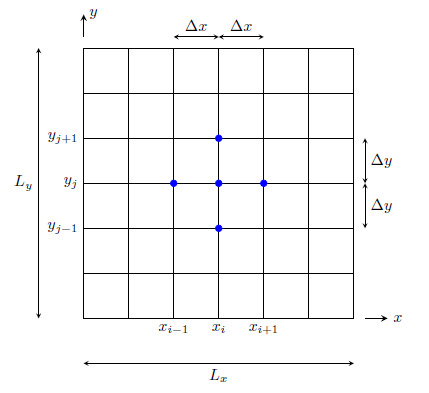
\includegraphics[width=0.8\textwidth]{Figures/finite_difference_picture.jpg}
    \caption{Finite Difference Mesh}
    \label{figure_1}
\end{figure}

Considering the orientation of adjacent nodes, all are expressed in terms of single location instead of two. This is done by utilizing the following equation, which is Equation \ref{equation_3}. 
\begin{equation} % 2D correspondence 
    n = j \times NX +i  
    \label{equation_3}
\end{equation}

After the mesh system is defined in a compact manner, certain parameters are defined in the following manner, as presented in Equation \ref{equation_4} and  \ref{equation_5}. 
\begin{equation} % 2D correspondence 
    \frac{\partial (uq)}{\partial x}_{i,j} \approx
\begin{cases}
    \frac{u(i, j)p(i, j) - u(i-1, j)q(i-1, j)}{x(i, j) - x(i-1, j)}, & \text{for } u(i, j) \geq 0 \\
    \frac{u(i+1, j)p(i+1, j) - u(i, j)q(i, j)}{x(i+1, j) - x(i, j)}, & \text{for } u(i, j) < 0
\end{cases}  
    \label{equation_4}
\end{equation}
\begin{equation}
\frac{\partial (vq)}{\partial x}_{i,j} \approx
\begin{cases}
    \frac{v(i, j)p(i, j) - v(i-1, j)q(i-1, j)}{y(i, j) - y(i-1, j)}, & \text{for } v(i, j) \geq 0 \\
    \frac{v(i+1, j)p(i+1, j) - v(i, j)q(i, j)}{y(i+1, j) - y(i, j)}, & \text{for } v(i, j) < 0
\end{cases}
\label{equation_5}
\end{equation}

Once $\frac{\partial (vq)}{\partial x}_{i,j}$ and $\frac{\partial (vq)}{\partial x}_{i,j}$ are defined, $\frac{\partial q}{\partial t}_{i,j}$ can be calculated using Equation \ref{equation_6}:             

\begin{equation} % 2D correspondence 
    \frac{\partial q}{\partial t} = \text{rhs}(q) = \left(-\frac{\partial (uq)}{\partial x} + \frac{\partial (vq)}{\partial y}\right) 
    \label{equation_6}
\end{equation}

Using all these definitions and variables, the solver is completed by the addition of the Runge-Kutta method. 
\label{solver_section}

\subsection{The Parallelization Using OpenMP}
The serial implementation of the solver is made according to the steps explained in Section \ref{solver_section}. In this section, the parallelization using OpenMP is explained. The main changes are made on the computationally intensive part of the solver, which is the "RhsQ" function. The integration method is kept the same, the only change is made in the structure of the processes. 

In the first step, the current and total core numbers are stored in a variable to be used later. In addition to these, the current node number is also calculated and stored in another variable. This calculation is explained in \ref{solver_section} and the related equation is given in Equation \ref{equation_3}. This part of parallel solver in the code file is given below: 
\definecolor{mygray}{rgb}{0.95,0.95,0.95}
\begin{minted}[autogobble=true, frame=lines, framesep=4mm, baselinestretch=1.2, bgcolor=mygray, fontsize=\footnotesize, linenos=true, breaklines]{c}
int my_rank = omp_get_thread_num();
int thread_count = omp_get_num_threads();
\end{minted}

\definecolor{mygray}{rgb}{0.95,0.95,0.95}
\begin{minted}[autogobble=true, frame=lines, framesep=4mm, baselinestretch=1.2, bgcolor=mygray, fontsize=\footnotesize, linenos=true, breaklines]{c}
for(int j=0; j<msh->NY; j++){
    for(int i=0; i<msh->NX; i++){
      const int idn = j*msh->NX + i; 
\end{minted}

At this point, it is important to notice that the calculation of current node number (idn) is performed under a loop. This reason of this is to consider whole space which is represented in terms of nodes. The operations on core numbers are outside the loop; however, this is not a problem as it will be later seen that this function will be called again and again by parallelizing in the main section of the code. 

The meaning of storing current and total core numbers appears here. In order to make parallel calculation in the related core, current node number (idn) is divided by total core number and the remainder is compared with the current core number. If this equality check returns true, then the operation is performed. Otherwise, the code moves on. This part of the code is given below: 

\definecolor{mygray}{rgb}{0.95,0.95,0.95}
\begin{minted}[autogobble=true, frame=lines, framesep=4mm, baselinestretch=1.2, bgcolor=mygray, fontsize=\footnotesize, linenos=true, breaklines]{c}
for(int j=0; j<msh->NY; j++){
    for(int i=0; i<msh->NX; i++){
      const int idn = j*msh->NX + i; 
      const double unx = solver->u[2*idn + 0];
      const double uny = solver->u[2*idn + 1];

      if ((idn % thread_count) == my_rank){ //paralel part

        // neighbor elements
        int elmE = msh->N2N[4*idn + 0];
        int elmN = msh->N2N[4*idn + 1];
        int elmW = msh->N2N[4*idn + 2];
        int elmS = msh->N2N[4*idn + 3];

        // neighbor velocities
        double uxE = solver->u[2*elmE + 0];
        double uyN = solver->u[2*elmN + 1];
        double uxW = solver->u[2*elmW + 0];
        double uyS = solver->u[2*elmS + 1];

        // Find spacing just in case it is not uniform
        double hip1 = fabs(msh->x[elmE] - msh->x[idn] ); 
        double him1 = fabs(msh->x[idn]  - msh->x[elmW]);  

        double hjp1 = fabs(msh->y[elmN] - msh->y[idn] );  
        double hjm1 = fabs(msh->y[idn]  - msh->y[elmS]);  

        double dfqdx = unx> 0 ? (unx*solver->q[idn]- uxW*solver->q[elmW])/him1 :  (uxE*solver->q[elmE]- unx*solver->q[idn])/hip1;
        double dfqdy = uny> 0 ? (uny*solver->q[idn]- uyS*solver->q[elmS])/hjm1 :  (uyN*solver->q[elmN]- uny*solver->q[idn])/hjp1;

        double rhsq   = -(dfqdx +dfqdy);

        // Time integration i.e. resq = rk4a(stage)* resq + dt*rhsq
        double resq = tstep->rk4a[stage]*tstep->resq[idn] + tstep->dt*rhsq; 
        // Update q i.e. q = q 6 rk4b(stage)*resq
        solver->q[idn]  +=  tstep->rk4b[stage]*resq;

        tstep->resq[idn] = resq; 
        tstep->rhsq[idn] = rhsq; 
      }
    }
  }
\end{minted}

This parallelized code is called in the main section by specifying parallel programming information beforehand. This specifications and the code are given below: 
\definecolor{mygray}{rgb}{0.95,0.95,0.95}
\begin{minted}[autogobble=true, frame=lines, framesep=4mm, baselinestretch=1.2, bgcolor=mygray, fontsize=\footnotesize, linenos=true, breaklines]{c}
//paralel programing information
  int thread_count;
  thread_count = strtol(argv[2], NULL, 10);
  omp_set_num_threads(thread_count);
\end{minted}

\definecolor{mygray}{rgb}{0.95,0.95,0.95}
\begin{minted}[autogobble=true, frame=lines, framesep=4mm, baselinestretch=1.2, bgcolor=mygray, fontsize=\footnotesize, linenos=true, breaklines]{c}
// ********************Time integration***************************************/
  // for every steps
  for(int step = 0; step<Nsteps; step++){
    // for every stage
    for(int stage=0; stage<tstep.Nstage; stage++){


      #pragma omp parallel 
        // Call integration function
        RhsQ(&advc, &tstep, stage); 
  
    }
\end{minted}

To record timings at the end of solving process a timer is initiated and later it is terminated. The elapsed time is calculated and stored in a variable. This implementation is also given below: 

\definecolor{mygray}{rgb}{0.95,0.95,0.95}
\begin{minted}[autogobble=true, frame=lines, framesep=4mm, baselinestretch=1.2, bgcolor=mygray, fontsize=\footnotesize, linenos=true, breaklines]{c}
// Start the timer
  double start_time = omp_get_wtime();
\end{minted}

\definecolor{mygray}{rgb}{0.95,0.95,0.95}
\begin{minted}[autogobble=true, frame=lines, framesep=4mm, baselinestretch=1.2, bgcolor=mygray, fontsize=\footnotesize, linenos=true, breaklines]{c}
// Stop the timer
double end_time = omp_get_wtime();

// Calculate and print the elapsed time
double elapsed_time = end_time - start_time;
\end{minted}

This completes the parallelization of a serial solver through OpenMP. To evaluate the performance of this solver, different resolutions are provided in the input file and corresponding timings are also recorded and they will be given in Section \ref{results_section}. 
\clearpage

\section{The Calculation of Infinity Norm }
\label{Inf_section}
Infinity norm simply indicates how large a vector is by comparing its magnitude with the largest entry. In the parallelized explicit in-time solver with finite difference solver, this norm can be found by three different methods. These methods belong to OpenMP, and they can be listed as "Critical Regions", "Atomic Operations" and "Reductions". All these methods have pros and cons compared to each other. However, in this text, the timing of computation is taken as base to evaluate their performance. 

These methods are applied as separate functions taking results of solver and performing comparison to obtain the infinity norm. The details of these functions will be provided throughout this section. 

\subsection{Critical Regions}
The logic behind using Critical Regions to find infinity norm is based on comparing the result of solver by a predefined value, then recording it to a variable if it is larger than this predefined value. In order to implement this on the main code, a function is created. At this point, it is important to make sure that this runs for every step and two values, current and predefined, are compared to each other. This is also ensured by the use of for loop.  

The problem with this method is the computational time. Since it makes the code more serial than it was, the computational time is more compared to atomic and reduction methods, which is less efficient. This will be also represented in Section \ref{results_section} in more detail. 
\definecolor{mygray}{rgb}{0.95,0.95,0.95}
\begin{minted}[autogobble=true, frame=lines, framesep=4mm, baselinestretch=1.2, bgcolor=mygray, fontsize=\footnotesize, linenos=true, breaklines]{c}
double inf_norm_C(solver_t *solver,double Val){
mesh_t *msh = &solver->msh;

double maxVal=Val;

#pragma omp parallel for shared(maxVal)
    for (int idn = 0; idn < msh->NX*msh->NY; idn++) {
      #pragma omp critical
      {
        if (solver->q[idn] > maxVal) {
          
                    maxVal = solver->q[idn];
                  }
                }
    }
return maxVal;
}
\end{minted}

\subsection{Atomic Operations}
Atomic Operations compensates the serialized effect of Critical Regions, so it is safer to use this to calculate infinity norm. However, it is possible to encounter hardware restrictions in the utilization of this method. The computational time is less compared to Critical Regions, so it is more efficient in that sense. 

\definecolor{mygray}{rgb}{0.95,0.95,0.95}
\begin{minted}[autogobble=true, frame=lines, framesep=4mm, baselinestretch=1.2, bgcolor=mygray, fontsize=\footnotesize, linenos=true, breaklines]{c}
double inf_norm_A(solver_t *solver, double Val) {
    mesh_t *msh = &solver->msh;

    #pragma omp parallel for
    for (int idn = 0; idn < msh->NX * msh->NY; idn++) {
      if (Val < solver->q[idn]){
        #pragma omp atomic write
        Val = solver->q[idn];
      }
      //else {
       // #pragma omp atomic write
       // Val = Val;
     // }
    }

    return Val;
}
\end{minted}

\subsection{Reductions}
Reductions are more preferred compared to other methods since it improves the parallelism characteristic. It is the one having the least computational time and also the most effective in that sense. 

\definecolor{mygray}{rgb}{0.95,0.95,0.95}
\begin{minted}[autogobble=true, frame=lines, framesep=4mm, baselinestretch=1.2, bgcolor=mygray, fontsize=\footnotesize, linenos=true, breaklines]{c}
double inf_norm_R(solver_t *solver,double Val){
mesh_t *msh = &solver->msh;
double maxVal=Val;
#pragma omp parallel for reduction(max:maxVal)
    for (int idn = 0; idn < msh->NX*msh->NY; idn++) {
        if (solver->q[idn] > maxVal) {
                    maxVal = solver->q[idn];
                }
    }
return maxVal;
}
\end{minted}

At this stage, it is important to point out the way followed to run the code using one of these options. The operation performed is specified by the input from the user. In that sense the following numbers are defined to represent four different options. \\ \\1: Only running parellel rshQ function \\
2: Infinity norm calculation with critical sections \\
3: Infinity norm calculation with reduction \\
4: Infinity norm calculation wih atomic \\

By specifying the desired number, the desired operation can be initiated. To compile the code and run the code, the followings should be made: 
\begin{itemize}
\color{black}
\item To compile the code: \colorbox{pink}{gcc -o advection advection.c -lm -fopenmp}
\item To run the code: \colorbox{pink}{./advection input.dat core-number desired-analysis}
\end{itemize}

\noindent
{\color{black} \rule{\linewidth}{0.5mm}}

\clearpage
\section{Results}
\label{results_section}
\subsection{Part 1: Parallelizations}
"How is parallelization applied" is explained in Section \ref{Theory_section}. In this section, the results are shown. As seen in Figure \ref{201*201_res}-\ref{401*401_res}-\ref{801*801_res}, also expected result is plotted. The expected result assumes that the main required time is 1 core computational time of that resolution. If the parallelization is 100\% efficient, then 2 cores computational time has to be half of 1 core computational time. This calculation is repeated for 3 and 4 cores computational time. 
\subsubsection{Recorded Timings for Different Mesh Resolutions}


\begin{figure}[hbt!]
  \centering
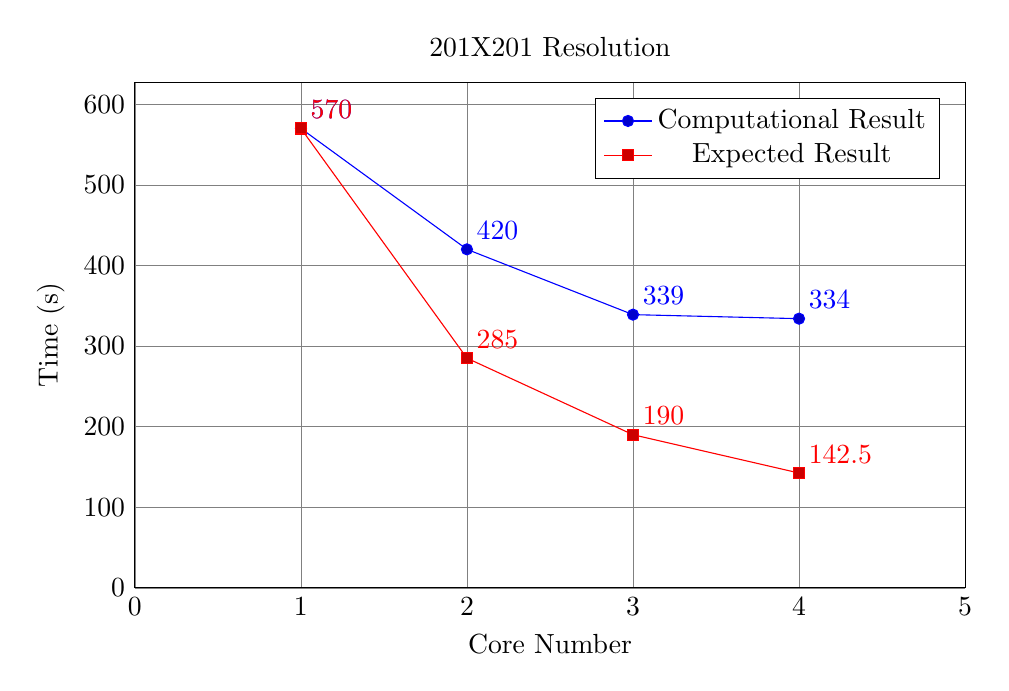
\begin{tikzpicture}
  \begin{axis}[
    width=1\linewidth, % Grafik genişliği belirle
    height=8cm, % Grafik yüksekliği belirle
    ylabel={Time (s)},
    xlabel={Core Number},
    title={201X201 Resolution},
    legend pos=north east, 
    grid=major, 
    xmin=0, xmax=5, % x ekseni limitleri
    ymin=0,
    xtick={0,1,2,3,4,5}, % x eksenindeki işaretler
    grid style={help lines}, % Izgara stilini belirle
  ]
  \addplot+[
    nodes near coords,
    nodes near coords align={above right}, % Değerleri sağ üst köşede göster
    point meta=explicit symbolic,
  ] coordinates {
    (1, 570) [570]
    (2, 420) [420]
    (3, 339) [339]
    (4, 334) [334]
  };
 \addlegendentry{Computational Result}
  \addplot+[
    nodes near coords,
    nodes near coords align={above right}, % Değerleri sağ üst köşede göster
    point meta=explicit symbolic,
  ] coordinates {
    (1, 570) [570]
    (2, 285) [285]
    (3, 190) [190]
    (4, 142.5) [142.5]
  };
 \addlegendentry{Expected Result}
  \end{axis}

\end{tikzpicture}
  \caption{Calculation results with the expected result for 201X201 resolution}
  \label{201*201_res}
\end{figure}


\begin{figure}[hbt!]
  \centering
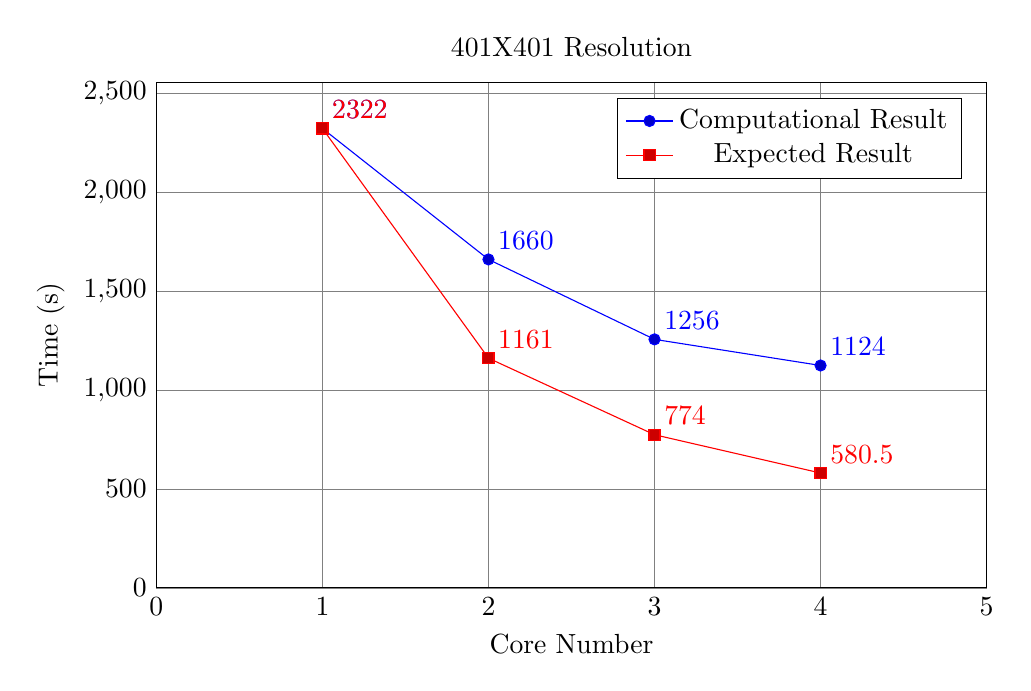
\begin{tikzpicture}
  \begin{axis}[
    width=1\linewidth, % Grafik genişliği belirle
    height=8cm, % Grafik yüksekliği belirle
    ylabel={Time (s)},
    xlabel={Core Number},
    title={401X401 Resolution},
    legend pos=north east, 
    grid=major, 
    xmin=0, xmax=5,
    ymin=0,
    xtick={0,1,2,3,4,5},
    grid style={help lines},
  ]
 
  \addplot+[
    nodes near coords,
    nodes near coords align={above right},
    point meta=explicit symbolic,
  ] coordinates {
    (1, 2322) [2322]
    (2, 1660) [1660]
    (3, 1256) [1256]
    (4, 1124) [1124]
  };
   \addlegendentry{Computational Result}
  \addplot+[
    nodes near coords,
    nodes near coords align={above right}, % Değerleri sağ üst köşede göster
    point meta=explicit symbolic,
  ] coordinates {
    (1, 2322) [2322]
    (2, 1161) [1161]
    (3, 774) [774]
    (4, 580.5) [580.5]
  };
 \addlegendentry{Expected Result}
  \end{axis}
\end{tikzpicture}
  \caption{Calculation results with the expected result for 401X401 resolution}
  \label{401*401_res}
\end{figure}


\begin{figure}[hbt!]
  \centering
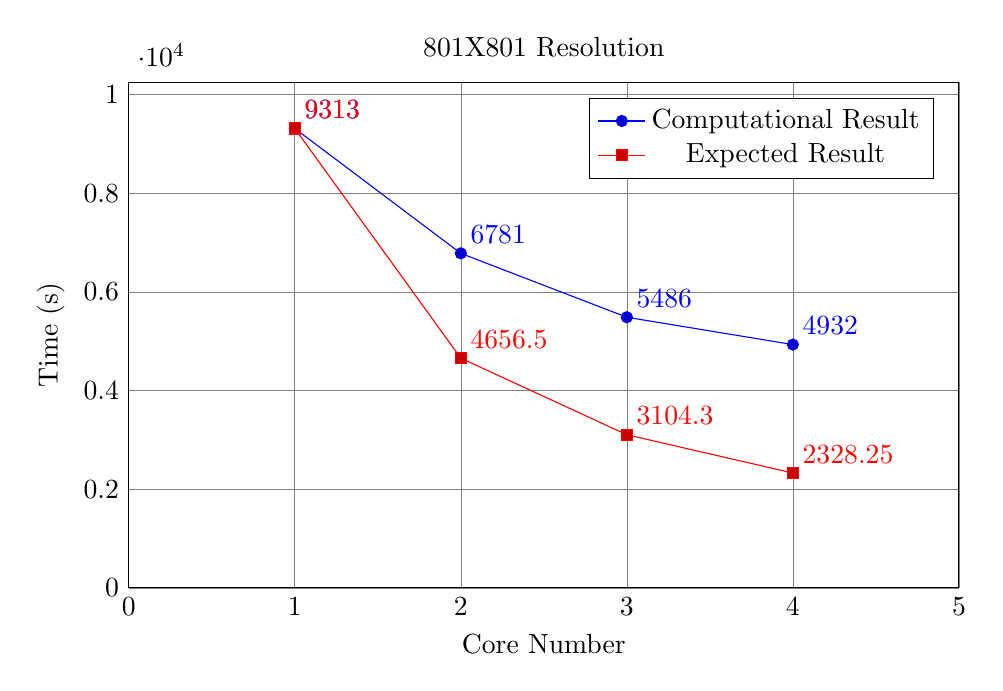
\begin{tikzpicture}
  \begin{axis}[
    width=1\linewidth, % Grafik genişliği belirle
    height=8cm, % Grafik yüksekliği belirle  
    ylabel={Time (s)},
    xlabel={Core Number},
    title={801X801 Resolution},
    legend pos=north east, 
    grid=major, 
    xmin=0, xmax=5,
    ymin=0,
    xtick={0,1,2,3,4,5},
    grid style={help lines},
  ]

    \addplot+[
    nodes near coords,
    nodes near coords align={above right},
    point meta=explicit symbolic,
  ] coordinates {
    (1, 9313) [9313]
    (2, 6781) [6781]
    (3, 5486) [5486]
    (4, 4932) [4932]
  };
   \addlegendentry{Computational Result}
  \addplot+[
    nodes near coords,
    nodes near coords align={above right}, % Değerleri sağ üst köşede göster
    point meta=explicit symbolic,
  ] coordinates {
    (1, 9313) [9313]
    (2, 4656.5) [4656.5]
    (3, 3104.3) [3104.3]
    (4, 2328.25) [2328.25]
  };
 \addlegendentry{Expected Result}
  \end{axis}
\end{tikzpicture}
  \caption{Calculation results with the expected result for 801X801 resolution}
  \label{801*801_res}
\end{figure}

\clearpage
\subsection{Part 2: Infinity Norms}
"How is the infinity norm calculated" is explained in Section\ref{Inf_section}. As seen in Figure\ref{inf_result}, the infinity norm is changed with a total number of nodes. This is expected due to the nature of the advection problem. If mesh resolution increases, critical regions are calculated more accurately. But these critical regions can be also singular points. So that if most part of the solution is not changed with increasing mesh resolution, the solution can be accepted.

\begin{figure}[hbt!]
  \centering
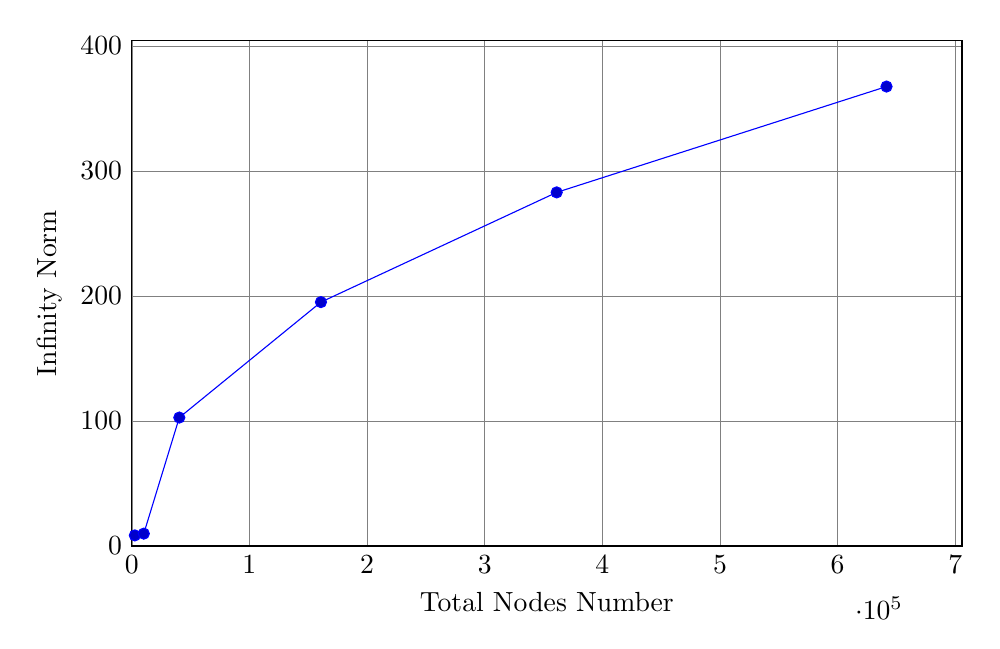
\begin{tikzpicture}
  \begin{axis}[
    width=1\linewidth, % Grafik genişliği belirle
    height=8cm, % Grafik yüksekliği belirle  
    ylabel={Infinity Norm},
    xlabel={Total Nodes Number},
    grid=major, 
    ymin=0,
    xmin=0,
    grid style={help lines},
  ]
\addplot coordinates {
  (2601, 8.49) 
  (10201, 9.89) 
  (40401, 102.72)
  (160801, 195.04) 
  (361201, 282.78) 
  (641601, 367.42)
  };
  \end{axis}
\end{tikzpicture}
  \caption{Infinity Norm Result of Different Total Nodes Number}
  \label{inf_result}
\end{figure}


In the next section, the times for calculating the infinity norm with three approaches are shown. Since every approach found the same result, the results are not shown again and can be seen in figure\ref{inf_result}. 

\clearpage
\subsubsection{Recorded Timings for Different Mesh Resolutions}

\begin{figure}[hbt!]
  \centering
\begin{tikzpicture}
  \begin{axis}[
    ybar,
    ylabel={Time (s)},
    title={Node Number 2601 (51*51)},
    width=1\linewidth,
    height=7.5cm,
    bar width=0.5,
    grid=major,
    symbolic x coords={atomic, critical, reduction},
    xtick=data,
    xticklabels={Atomic Method, Critical Method, Reduction Method}, % X eksenindeki etiketleri büyük harfle başlat
    nodes near coords,
    nodes near coords align={above},
    ymin=0,
  ]
  
  \addplot coordinates {(atomic, 26.55) (critical, 42.26) (reduction, 27.35)};
  
  \end{axis}
\end{tikzpicture}
  \caption{Required time for 51x51 mesh resolution with three parallelization approach}
  \label{inf_result_051}
\end{figure}


\begin{figure}[hbt!]
  \centering
\begin{tikzpicture}
  \begin{axis}[
    ybar,
    ylabel={Time (s)},
    title={Node Number 10201 (101*101)},
    width=1\linewidth,
    height=7.5cm,
    bar width=0.5,
    grid=major,
    symbolic x coords={atomic, critical, reduction},
    xtick=data,
    xticklabels={Atomic Method, Critical Method, Reduction Method}, % X eksenindeki etiketleri büyük harfle başlat
    nodes near coords,
    nodes near coords align={above},
    ymin=0,
  ]
  
  \addplot coordinates {(atomic, 94.17) (critical, 158.11) (reduction, 94.9)};
  
  \end{axis}
\end{tikzpicture}
  \caption{Required time for 101x101 mesh resolution with three parallelization approach}
  \label{inf_result_101}
\end{figure}


\begin{figure}[hbt!]
  \centering
\begin{tikzpicture}
  \begin{axis}[
    ybar,
    ylabel={Time (s)},
    title={Node Number 40401 (201*201)},
    width=1\linewidth,
    height=8cm,
    bar width=0.5,
    grid=major,
    symbolic x coords={atomic, critical, reduction},
    xtick=data,
    xticklabels={Atomic Method, Critical Method, Reduction Method}, % X eksenindeki etiketleri büyük harfle başlat
    nodes near coords,
    nodes near coords align={above},
    ymin=0,
  ]
  
  \addplot coordinates {(atomic, 297.92) (critical, 552.22) (reduction, 300.7)};
  
  \end{axis}
\end{tikzpicture}
  \caption{Required time for 201x201 mesh resolution with three parallelization approach}
  \label{inf_result_201}
\end{figure}


\begin{figure}[hbt!]
  \centering
\begin{tikzpicture}
  \begin{axis}[
    ybar,
    ylabel={Time (s)},
    title={Node Number 160801 (401*401)},
    width=1\linewidth,
    height=8cm,
    bar width=0.5,
    grid=major,
    symbolic x coords={atomic, critical, reduction},
    xtick=data,
    xticklabels={Atomic Method, Critical Method, Reduction Method}, % X eksenindeki etiketleri büyük harfle başlat
    nodes near coords,
    nodes near coords align={above},
    ymin=0,
  ]
  
  \addplot coordinates {(atomic, 1270.62) (critical, 1943.92) (reduction, 1178.58)};
  
  \end{axis}
\end{tikzpicture}
  \caption{Required time for 401x401 mesh resolution with three parallelization approach}
  \label{inf_result_401}
\end{figure}


\begin{figure}[hbt!]
  \centering
\begin{tikzpicture}
  \begin{axis}[
    ybar,
    ylabel={Time (s)},
    title={Node Number 361201 (601*601)},
    width=1\linewidth,
    height=8cm,
    bar width=0.5,
    grid=major,
    symbolic x coords={atomic, critical, reduction},
    xtick=data,
    xticklabels={Atomic Method, Critical Method, Reduction Method}, % X eksenindeki etiketleri büyük harfle başlat
    nodes near coords,
    nodes near coords align={above},
    ymin=0,
  ]
  
  \addplot coordinates {(atomic, 2843.42) (critical, 5070) (reduction, 2778)};
  
  \end{axis}
\end{tikzpicture}
  \caption{Required time for 601x601 mesh resolution with three parallelization approach}
  \label{inf_result_601}
\end{figure}


\begin{figure}[hbt!]
  \centering
\begin{tikzpicture}
  \begin{axis}[
    ybar,
    ylabel={Time (s)},
    title={Node Number 641601 (801*801)},
    width=1\linewidth,
    height=8cm,
    bar width=0.5,
    grid=major,
    symbolic x coords={atomic, critical, reduction},
    xtick=data,
    xticklabels={Atomic Method, Critical Method, Reduction Method}, % X eksenindeki etiketleri büyük harfle başlat
    nodes near coords,
    nodes near coords align={above},
    ymin=0,
  ]
  
  \addplot coordinates {(atomic, 4849.79) (critical, 8698.23) (reduction, 4857.74)};
  
  \end{axis}
\end{tikzpicture}
  \caption{Required time for801x801 mesh resolution with three parallelization approach}
  \label{inf_result_801}
\end{figure}



\clearpage
\section{Conclusion and Comments}

In conclusion, in this paper, the effect of parallelization on a serialized solver is represented by considering the recorded timings. To evaluate the performance, the solver is run for different mesh resolutions and thread numbers. Infinity norm is also found by using the parallel code along with three different methods. These methods are critical regions, atomic and reductions. The methodology is explained and the results are presented throughout the paper. 

As seen in figures \ref{201*201_res}-\ref{401*401_res}-\ref{801*801_res}, parallelization is never 100\% percent efficient. This is expected because only the solver part is parallelized. Also, there are lot of communication time in solver. This problem cannot be solved with parallelization. However, as a general comment, it can be said that increasing the number of threads reduces the computation time, which is a desirable outcome. This amount of reduction does not match with the theoretical amount, which can be explained considering external effects such as hardware capability and the nature of solver. 

As seen in figure\ref{inf_result}, the infinity norm has not converged yet even though the mesh resolution is very high. This makes us think there can be singular points in the system. The infinity norm position and time have to be checked.   

As seen in figure \ref{inf_result_051}-\ref{inf_result_101}-\ref{inf_result_201}-\ref{inf_result_401}-\ref{inf_result_601}-\ref{inf_result_801}, required time for atomic and reduction methods are almost same. However, the required time for critical regions method is always higher than others. This is expected indeed since critical regions method makes the code similar to the serialized one due to its nature. 

\clearpage
\printbibliography

\end{document}
